\vspace{10pt}

{\centering\subsection*{梁好:游隐水洞}}

\addcontentsline{toc}{subsection}{梁好:游隐水洞}

\renewcommand{\leftmark}{梁好:游隐水洞}

\begin{figure}[htbp]

\centering

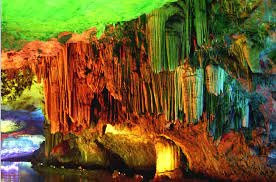
\includegraphics[width = .5\textwidth]{./ch/29.jpg}

\end{figure}



说到景点,大家定见过不少山、树木、森林、花、大海……今天我就带大家看看隐水洞的风光吧!


通山大约行了九公里后,到了隐水洞。只见隐水洞一路上人山人海,真不知是怎样的美景能吸引这么多人过去参观。我抱着这样好奇的心情来到了隐水洞洞口,只见那洞口像桥洞似的很宽。


我走进洞里后,只见彩灯照映在石壁上,让石头变成了五颜六色的“五彩石”,漂亮极了!


我们顺着工人的指点向北走,这时我看到一条壮观的瀑布出现在眼前。瀑布是从高处的缝里流下来的,这时我只能用李白的诗句《望庐山瀑布》中的“飞流直下三千尺,疑是银河落九天”来形容我眼前的壮观景象了。


参观完瀑布后我们再向北走,只见很多奇奇怪怪的溶石出现在面前。我顺着工作人员的指点看,那些形态各异的石钟乳和石笋看起来有像神仙的,大象的,小狗的……

看完溶石再向东北方向走,你会看到一条很长的河流,河流旁停靠着一条船,坐上船后,船快速的开动着,有点冷,这时周围激起了层层浪花,把手放上去,还会触到浪花呢!


船到站后,便来到了出口前,这时我只见到了一大群黑色蝙蝠在洞口上方的石壁上吊着,这时我的心都提到了嗓子眼,我吓坏了。我眯着眼睛像猫一样悄咪咪的走出洞口,虽然我已经走出了洞口,但我的心里还是像有十五只吊桶在打水——七上八下的,久久不能平静。



 隐水洞到处都有美丽的景色,说也说不尽,希望你有机会去细细游赏。


\vspace{10pt}

作者:四(1)班  梁好



指导老师:周瑞





投稿:2021年4月29日



发表:2021年5月7日














\vspace{10pt}

\hline



